
\documentclass[tikz]{standalone}
\begin{document}
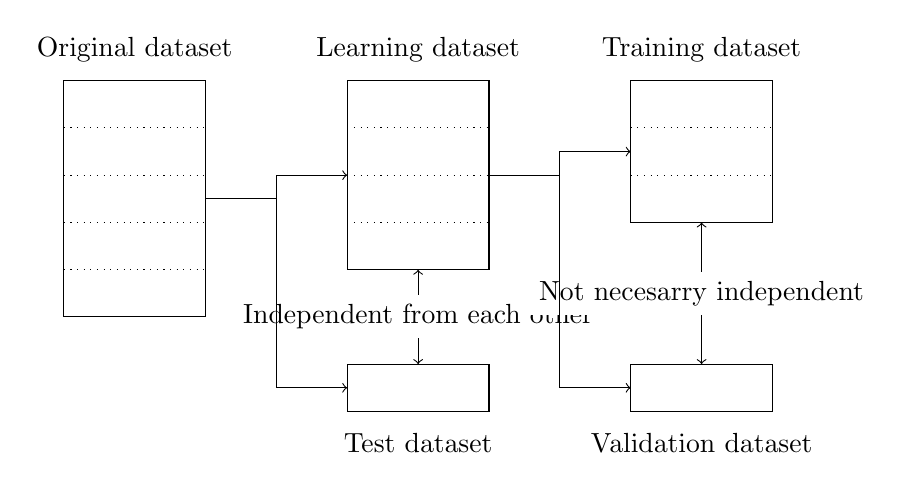
\begin{tikzpicture}
% 元データ
\draw (0,18mm) rectangle (18mm,48mm);
\node[] at (9mm,52mm) {Original dataset};

% 学習データ
\draw (36mm,24mm) rectangle (54mm,48mm);
\node[] at (45mm,52mm) {Learning dataset};

% テストデータ
\draw (36mm,6mm) rectangle (54mm,12mm);
\node[] at (45mm,2mm) {Test dataset};

% トレーニングデータ
\draw (72mm,30mm) rectangle (90mm,48mm);
\node[] at (81mm,52mm) {Training dataset};

% バリデーションデータ
\draw (72mm,6mm) rectangle (90mm,12mm);
\node[] at (81mm,2mm) {Validation dataset};

% 学習--テスト
\draw[<->] (45mm,12mm)--(45mm,24mm);
\node[fill=white] at (45mm,18mm) {Independent from each other};

% トレーニング--バリデーション
\draw[<->] (81mm,12mm)--(81mm,30mm);
\node[fill=white] at (81mm,21mm) {Not necesarry independent};

% 1--2カラム
\draw[->](18mm,33mm)--(27mm,33mm)--(27mm,36mm)--(36mm,36mm);
\draw[->](27mm,33mm)--(27mm,9mm)--(36mm,9mm);

% 2--3カラム
\draw[->](54mm,36mm)--(63mm,36mm)--(63mm,39mm)--(72mm,39mm);
\draw[->](63mm,36mm)--(63mm,9mm)--(72mm,9mm);

% 点線
\draw[dotted] (0mm,24mm)--(18mm,24mm);
\draw[dotted] (0mm,30mm)--(18mm,30mm);
\draw[dotted] (0mm,36mm)--(18mm,36mm);
\draw[dotted] (0mm,42mm)--(18mm,42mm);

\draw[dotted] (36mm,30mm)--(54mm,30mm);
\draw[dotted] (36mm,36mm)--(54mm,36mm);
\draw[dotted] (36mm,42mm)--(54mm,42mm);

\draw[dotted] (72mm,36mm)--(90mm,36mm);
\draw[dotted] (72mm,42mm)--(90mm,42mm);\end{tikzpicture}
\end{document}

